
\begin{frame}
\frametitle{Goals}
%\framesubtitle{Characteristics}
\begin{table}
\begin{tabular}{p{7cm}p{3cm}}
\begin{itemize}
  \item Analize the security risks in using username/password identification in P2P networks. 
  \item Check the different security schemes that can be used in a P2P network with malicious nodes.
  \item Propose a P2P username/password identification system.
\end{itemize}
&
\vspace{1.5cm}
%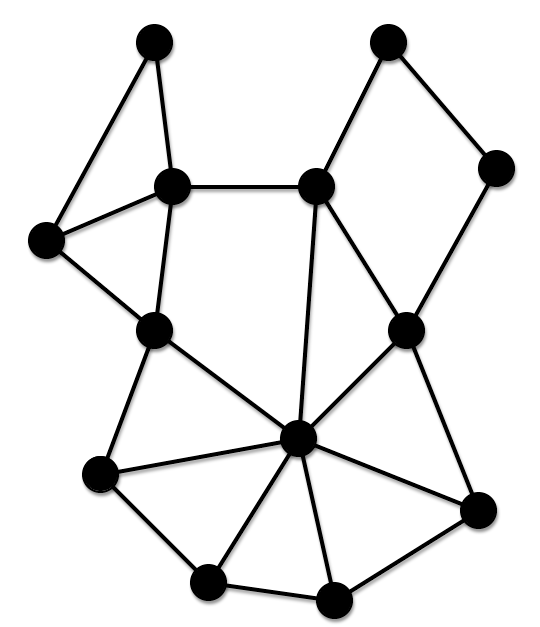
\includegraphics[width=4cm]{img/p2p-unstructured}\\
\end{tabular}
\end{table}
\end{frame}


\begin{frame}
\frametitle{P2P Networks}
\framesubtitle{Characteristics}
\begin{table}
\begin{tabular}{p{7cm}p{3cm}}
\begin{itemize}
  \item Scalable
  \item Decentralized
  \item Self-maintained
  \item Robust
\end{itemize}
&
\vspace{1.5cm}
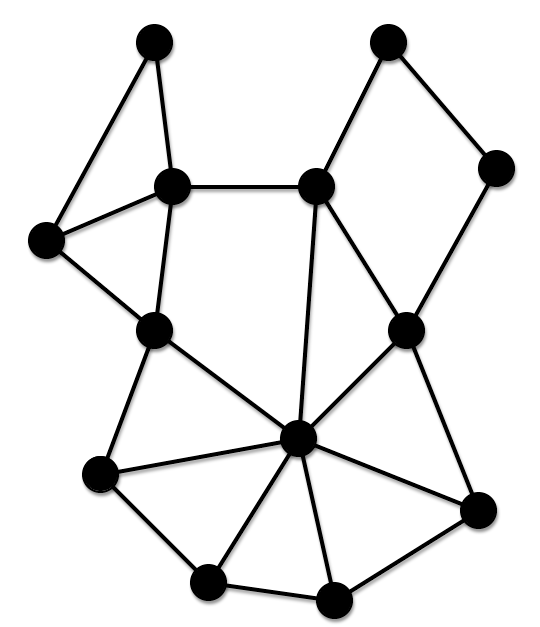
\includegraphics[width=4cm]{img/p2p-unstructured}\\
\end{tabular}
\end{table}
\end{frame}

\begin{frame}
\frametitle{P2P Networks}
\framesubtitle{Overlay structure}
\begin{table}
\begin{tabular}{p{7cm}p{3cm}}
\begin{itemize}
    \item Structured networks (CAN, CHORD)
    \item Unstructured networks (Gnutella, Bittorrent)
\end{itemize}
&
\vspace{1.5cm}
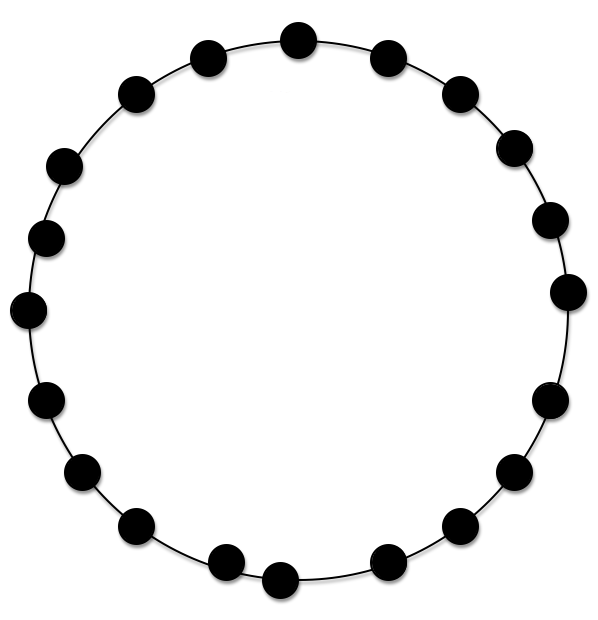
\includegraphics[width=4cm]{img/p2p-structured}\\
\end{tabular}
\end{table}
\end{frame}

\begin{frame}
\frametitle{P2P Networks}
\framesubtitle{Overlay structure}
\begin{table}
\begin{tabular}{p{7cm}p{3cm}}
\begin{itemize}
    \item Images of structured/unstructures networks
    \item Differences
\end{itemize}
&
\vspace{1.5cm}

\includegraphics[width=4cm]{img/example}\\
\end{tabular}
\end{table}
\end{frame}

\begin{frame}
\frametitle{Username / password identification}
\framesubtitle{Why?}
\begin{table}
\begin{tabular}{p{7cm}p{3cm}}
\begin{itemize}
  \item Many \b{complex systems} require authenticated users to work.
  \item Most of the users has \b{more than one device}, so identification through
    multiple devices is needed.
  \item \b{User are accostumed} to username/password solutions.
\end{itemize}
&
\vspace{1.5cm}
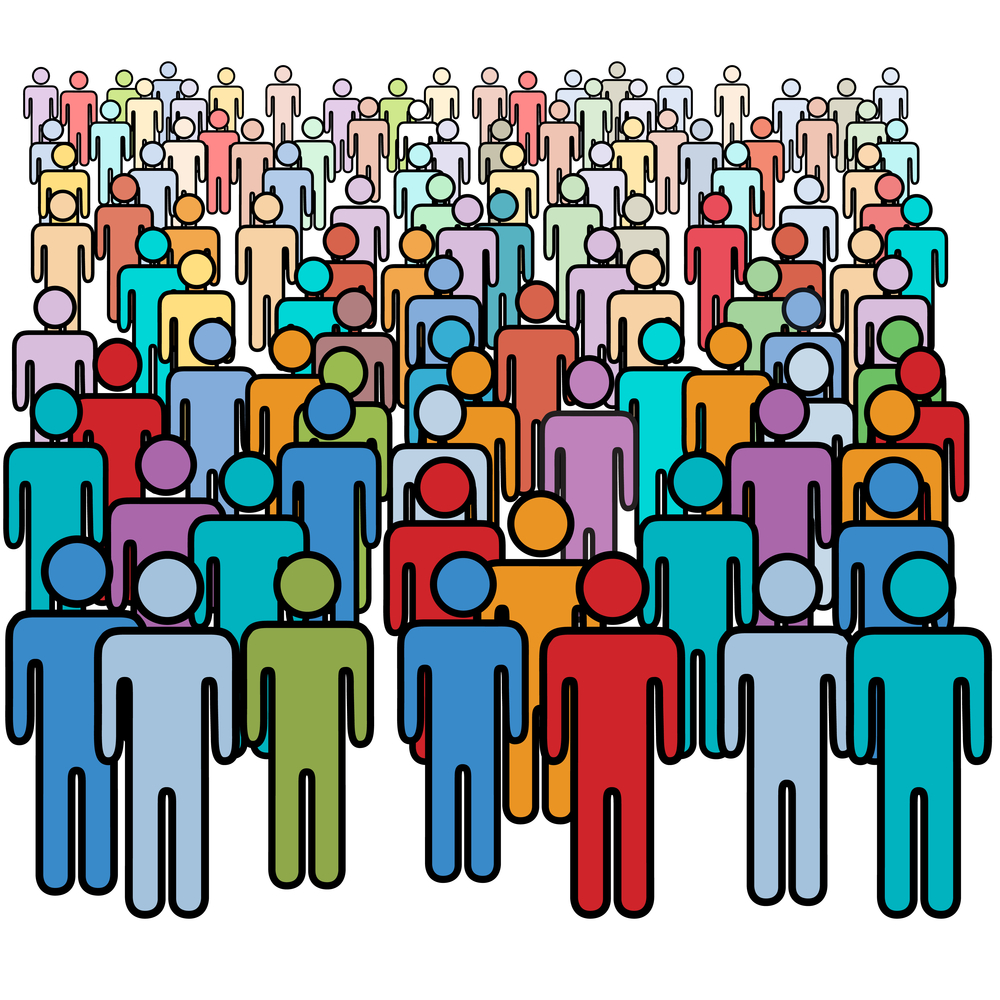
\includegraphics[width=4cm]{img/users}\\
\end{tabular}
\end{table}
\end{frame}

\begin{frame}
\frametitle{Username / password identification}
\framesubtitle{P2P Identification Schemes}

  Descentralized schemes distributes the task of public key auth to all
  participants.
\begin{table}
\begin{tabular}{p{7cm}p{3cm}}
\begin{itemize}
  \item PGP-like scheme\\ Creates web of trust to auth public keys based on
    their acquaintances opinions.
  \item Quorum-based scheme\\ Multiple independent participants replicate
    public keys.
\end{itemize}
&
\vspace{1.5cm}
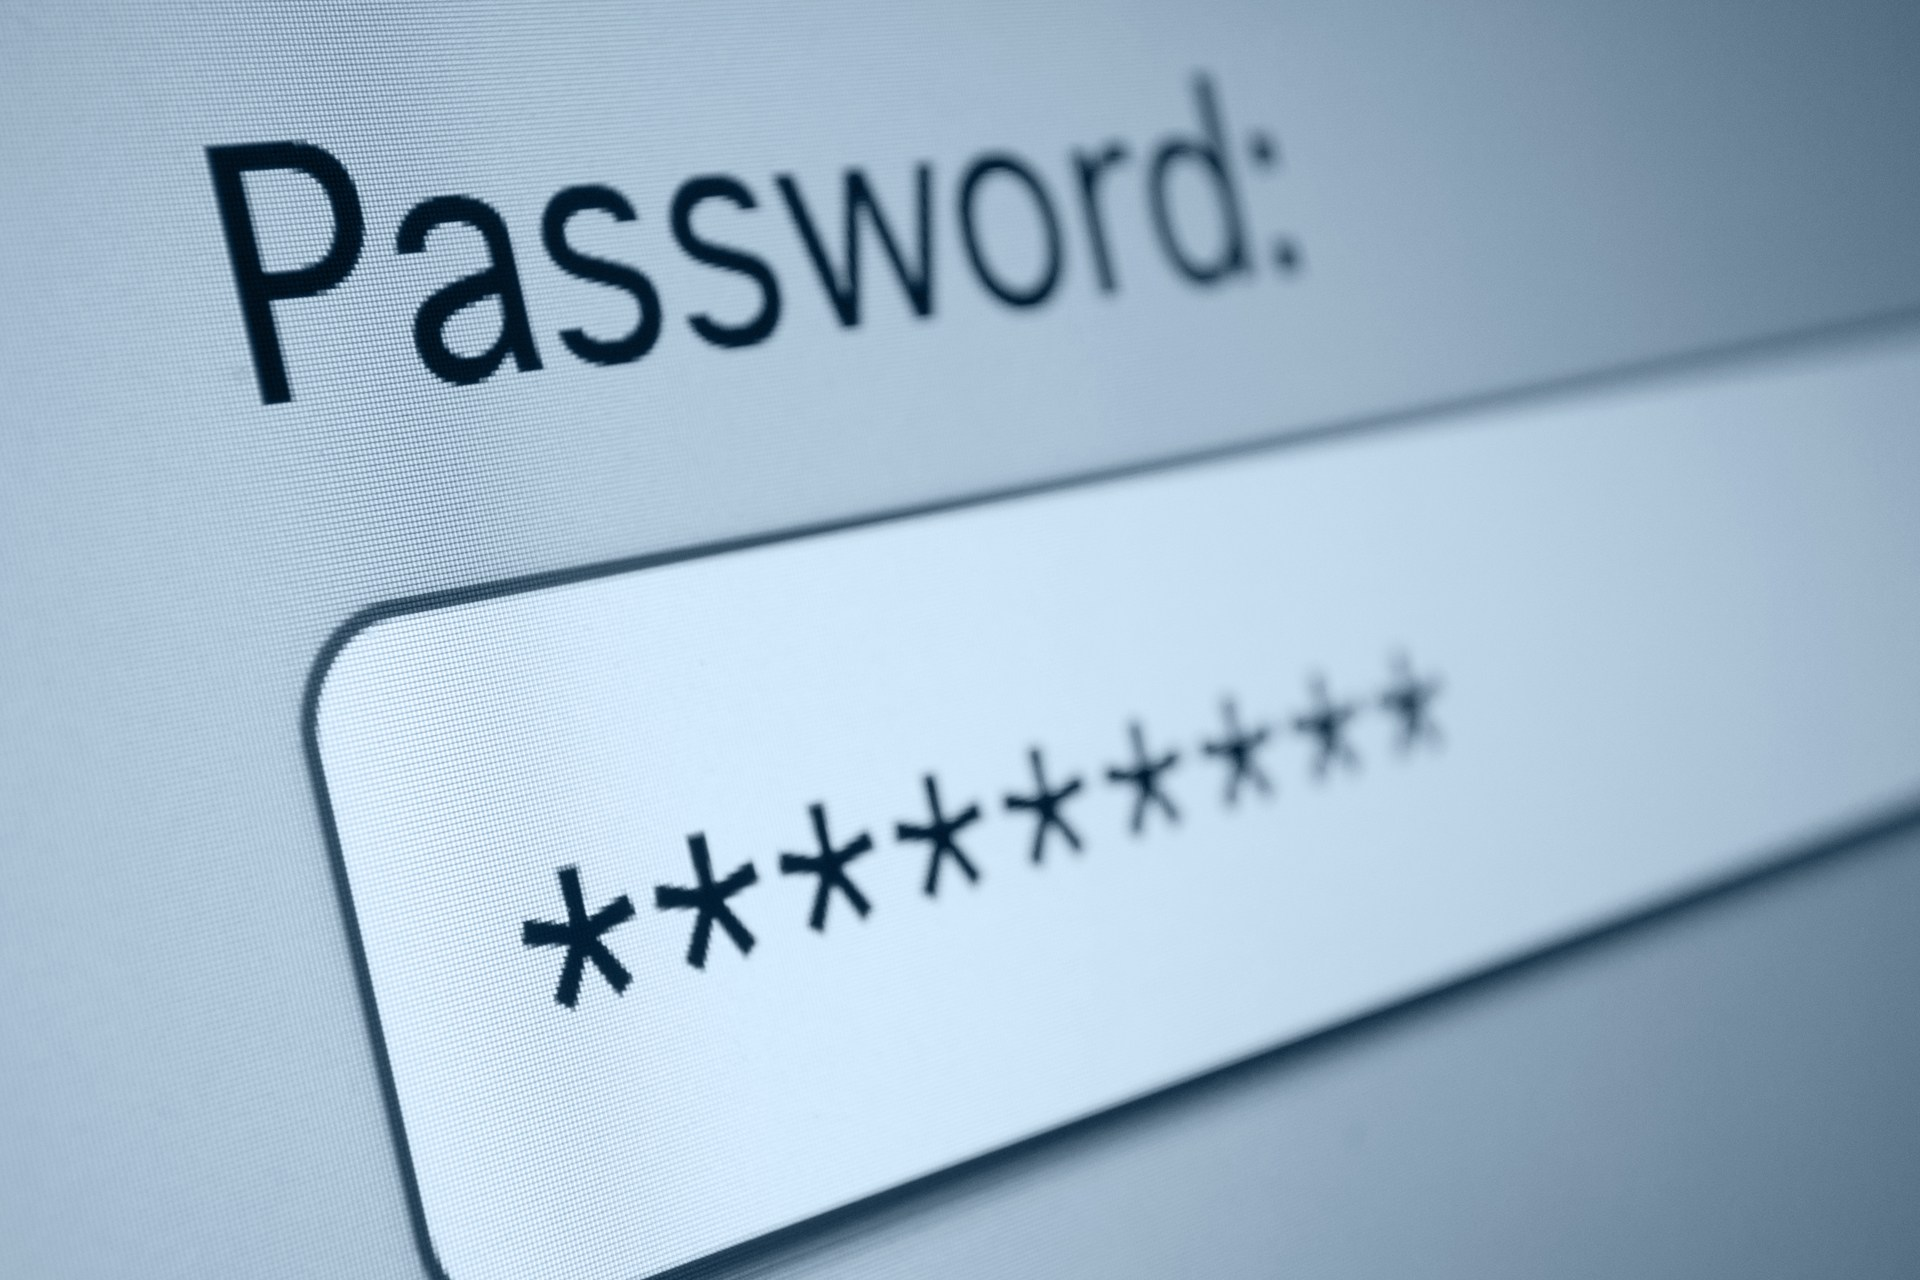
\includegraphics[width=4cm]{img/password}\\
\end{tabular}
\end{table}
\end{frame}

\begin{frame}
\frametitle{Identification schemes}
\framesubtitle{In need of a third party}
\begin{table}
\begin{tabular}{p{7cm}p{3cm}}
\begin{itemize}
    \item PKI
    \item Username/password pair
\end{itemize}

Poor scaling, single point of failure, heavy administration overhead.
&
\vspace{1.5cm}

\includegraphics[width=4cm]{img/keyboard_key}\\
\end{tabular}
\end{table}
\end{frame}

\begin{frame}
\frametitle{Trust in P2P networks}
\begin{table}
\begin{tabular}{p{7cm}p{3cm}}
\begin{enumerate}
    \item To deliver a valuable service in P2P applications, it
is important to trust that the participants will act as requested.
    \item We need to be sure that other peers will forward
messages, and that the designated peers will indeed save the information
correctly so that operations can be successful.
\end{enumerate}
&
\vspace{1.5cm}
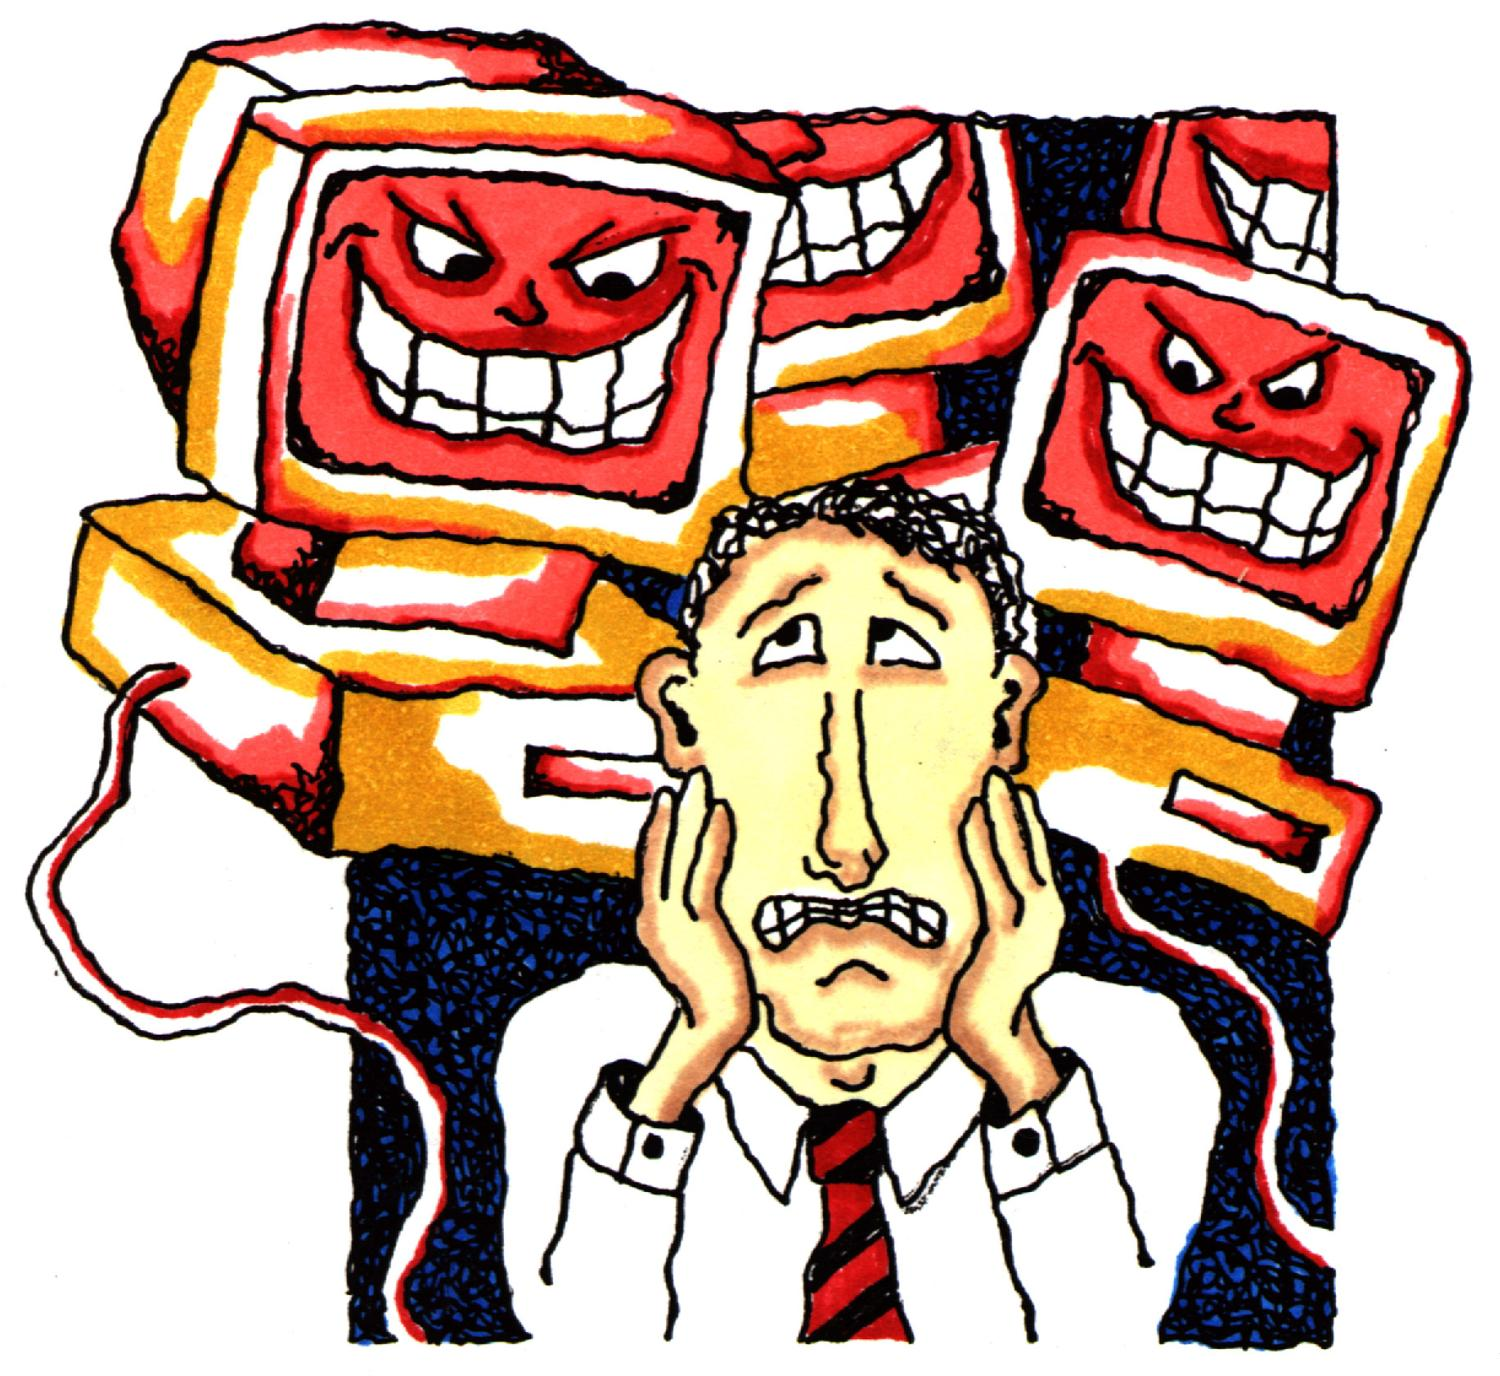
\includegraphics[width=4cm]{img/malicious}\\
\end{tabular}
\end{table}
\end{frame}

\begin{frame}
\frametitle{Trust in P2P networks}
\framesubtitle{Building Trust}
%Consequently, the quality of service of applications may
%be deteriorated due to message overhead or data loss.
\begin{table}
\begin{tabular}{p{7cm}p{3cm}}
\begin{enumerate}
    \item Complex since a P2P network includes untrusted nodes from an open environment.
    \item Untrusted nodes may be faulty, malicious, and act together to attack the network.
\end{enumerate}
&
\vspace{1.5cm}
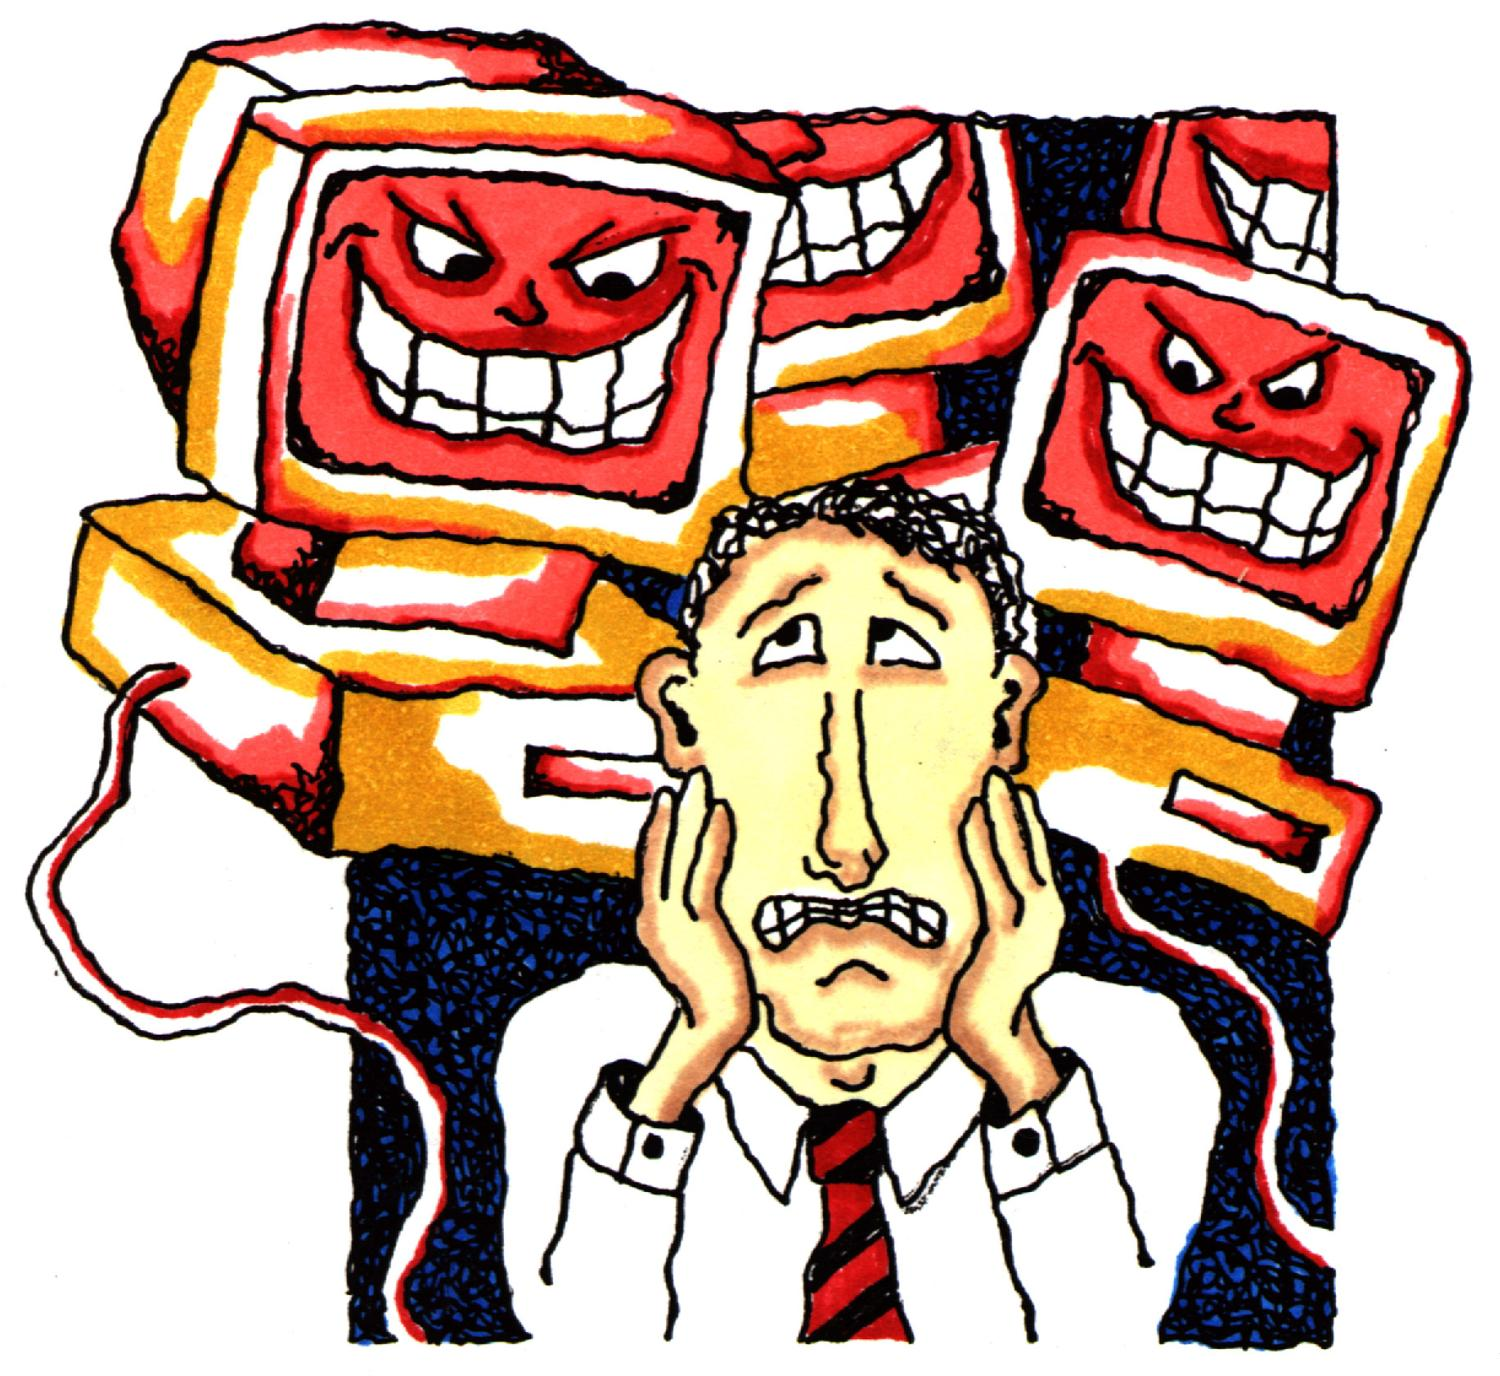
\includegraphics[width=4cm]{img/malicious}\\
\end{tabular}
\end{table}
\end{frame}

\begin{frame}
\frametitle{Trust in P2P networks}
\framesubtitle{How to detect faulty nodes?}
%Consequently, the quality of service of applications may
%be deteriorated due to message overhead or data loss.
\begin{table}
\begin{tabular}{p{7cm}p{3cm}}
\begin{description}
    \item{Reputation systems:} Assess the past history of a
peer by gathering feedback from nodes with previous interactions with this
peer.
    \item{Accountability:} Detects and exposes faulty nodes by
creating non-repudiable records of every node’s actions.
\end{description}
&
\vspace{1.5cm}
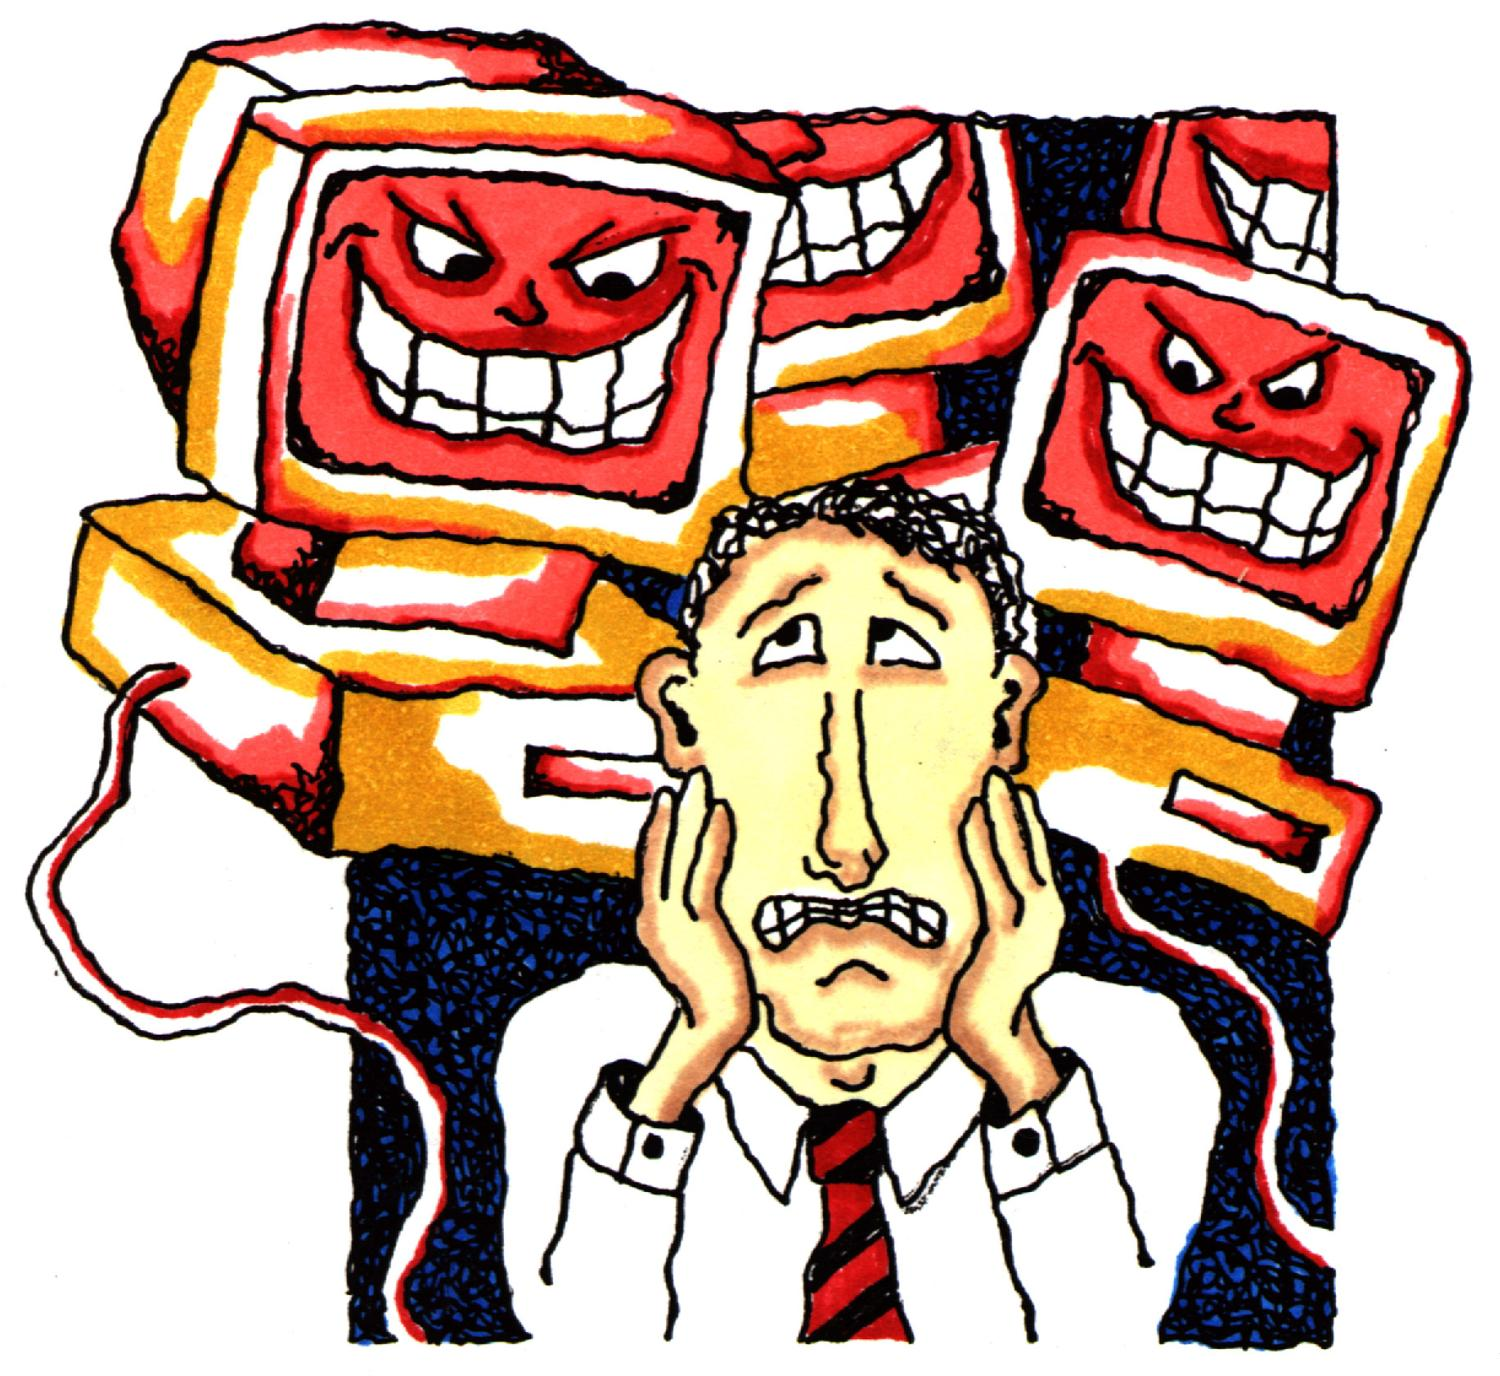
\includegraphics[width=4cm]{img/malicious}\\
\end{tabular}
\end{table}
\end{frame}

\begin{frame}
\frametitle{Trust in P2P networks}
\framesubtitle{Bizantine nodes}
\begin{table}
\begin{tabular}{p{7cm}p{3cm}}
Are all nodes that not behave as expected
%Multiples causes: connection problems, viruses, modified software, etc.\\
%\b{\*Nobody can be trusted}
\begin{enumerate}
    \item Faulty nodes
    \item Malicious nodes
    \item Infected nodes
\end{enumerate}
&
\vspace{1.5cm}
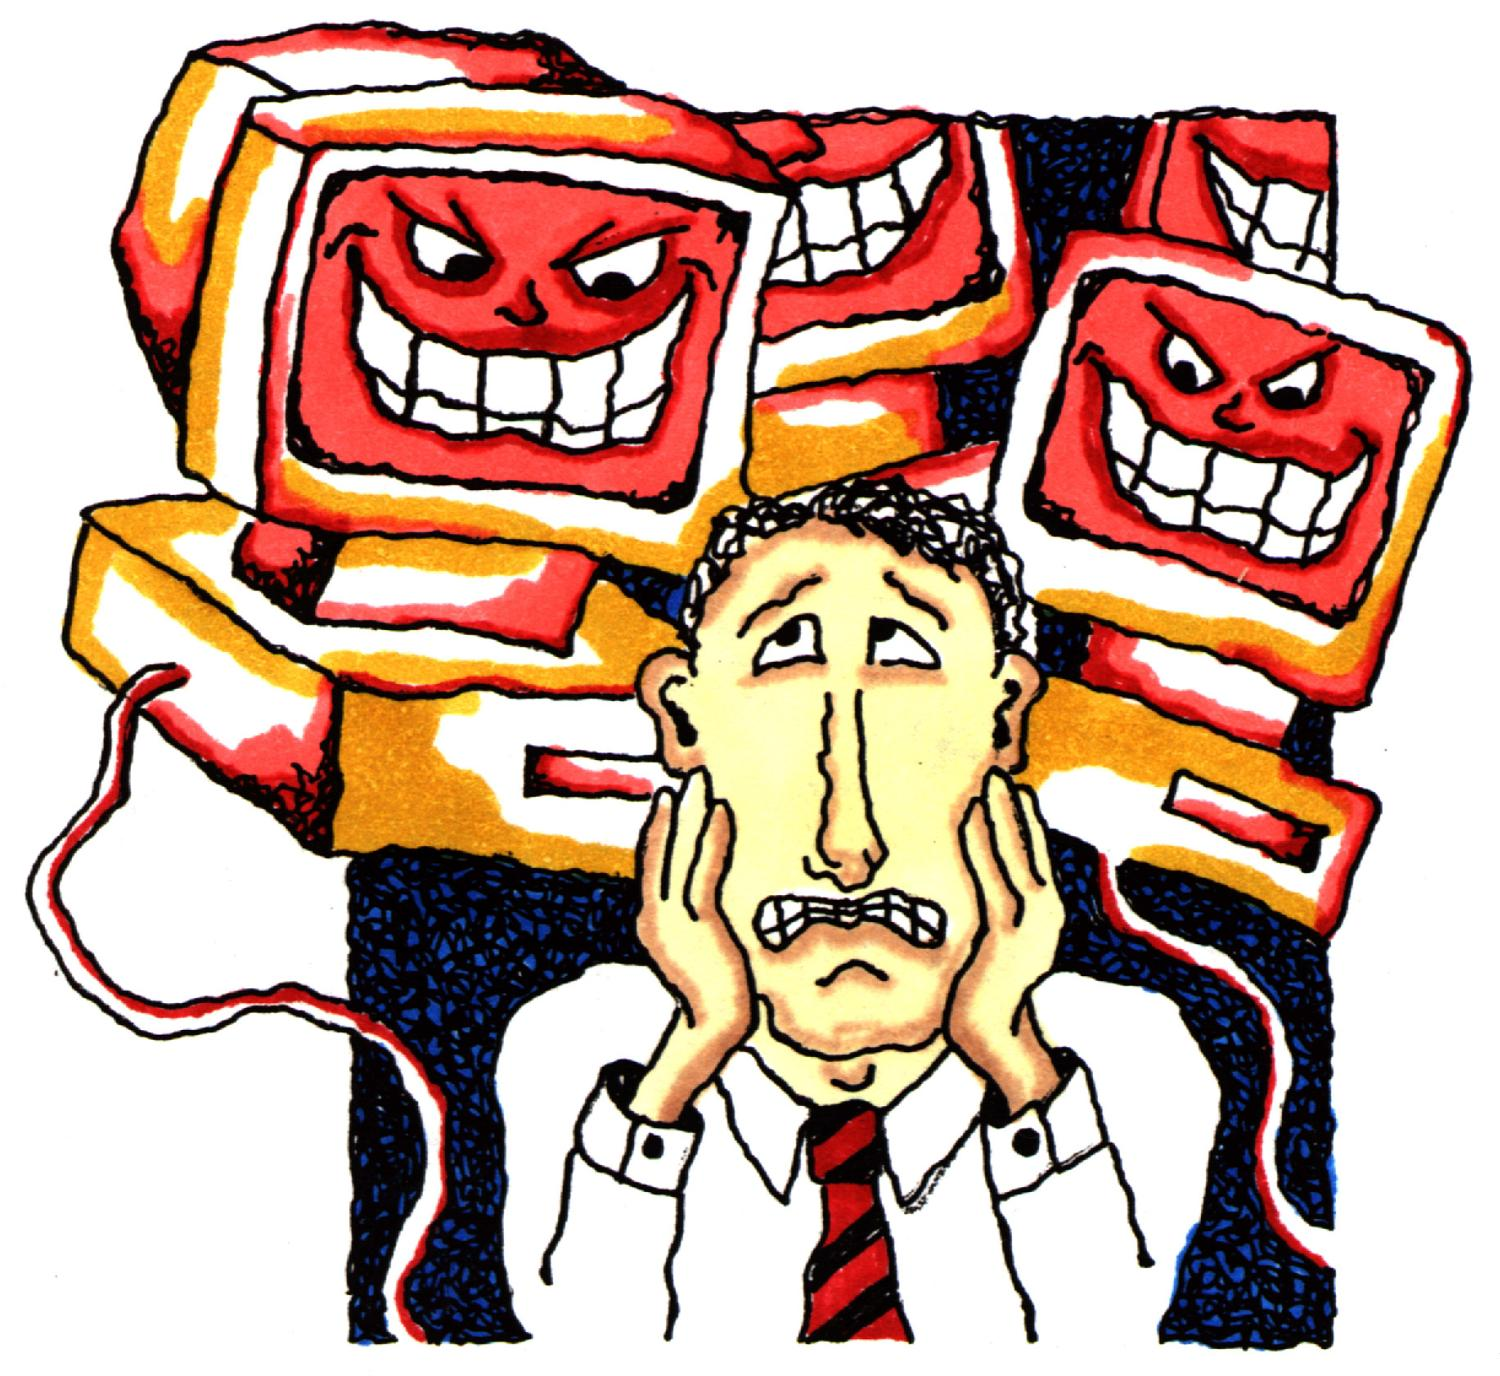
\includegraphics[width=4cm]{img/malicious}\\
\end{tabular}
\end{table}
\end{frame}

\begin{frame}
\frametitle{Trust in P2P networks}
\framesubtitle{Bizantine node tolerance}
\begin{table}
\begin{tabular}{p{7cm}p{3cm}}
  P2P networks can achieve byzantine fault tolerance under $1/3$ byzantine
  peers\\
  A peer is honest only if the peers executes the protocol faithfully;
  otherwise, the peer is faulty.
&
\vspace{1.5cm}
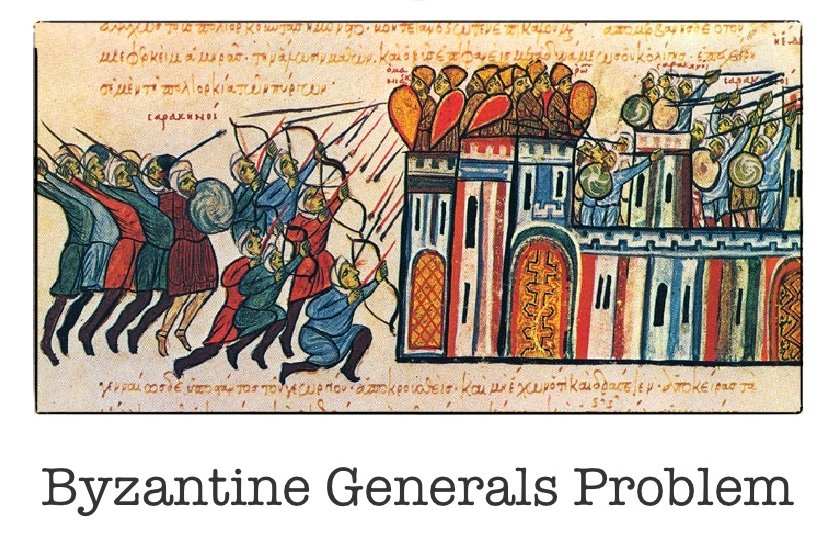
\includegraphics[width=4cm]{img/bizantine_generals_problem}\\
\end{tabular}
\end{table}
\end{frame}


\begin{frame}
\frametitle{Trust in P2P networks}
\framesubtitle{Bizantine node tolerance}
\begin{table}
\begin{tabular}{p{7cm}p{3cm}}
  P2P networks can achieve byzantine fault tolerance under $1/3$ byzantine
  peers\\
  A peer is honest only if the peers executes the protocol faithfully;
  otherwise, the peer is faulty.
&
\vspace{1.5cm}
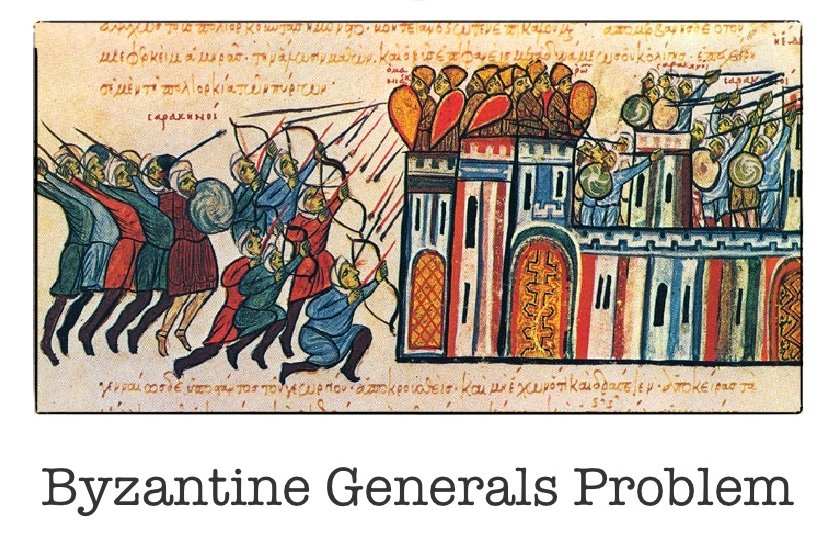
\includegraphics[width=4cm]{img/bizantine_generals_problem}\\
\end{tabular}
\end{table}
\end{frame}

